\documentclass{article}
\usepackage{ctex}
\usepackage{color}
\usepackage{listings}
\usepackage{graphicx}
\usepackage{float}
\usepackage{subfig}
\usepackage{overpic}
\lstset{ %
basicstyle=\footnotesize,       % the size of the fonts that are used for the code
numbers=left,                   % where to put the line-numbers
numberstyle=\footnotesize,      % the size of the fonts that are used for the line-numbers
stepnumber=1,                   % the step between two line-numbers. If it is 1 each line will be numbered
numbersep=5pt,                  % how far the line-numbers are from the code
backgroundcolor=\color{white},  % choose the background color. You must add \usepackage{color}
showspaces=false,               % show spaces adding particular underscores
showstringspaces=false,         % underline spaces within strings
showtabs=false,                 % show tabs within strings adding particular underscores
frame=single,           % adds a frame around the code
tabsize=2,          % sets default tabsize to 2 spaces
captionpos=b,           % sets the caption-position to bottom
breaklines=true,        % sets automatic line breaking
breakatwhitespace=false,    % sets if automatic breaks should only happen at whitespace
}

\title{\heiti Validation Document For Painkiller Injection System}
\author{%
  Panxin Tao, Runkang Yang, Zhekai Zhang\\
  SIST, ShanghaiTech University\\
  \texttt{taopx2022@shanghaitech.edu.cn}\\
  \texttt{yangrk2022@shanghaitech.edu.cn}\\
  \texttt{zhangzhk2022@shanghaitech.edu.cn}\\
}
\date{June 2024}
\begin{document}
\maketitle
\newpage
\section{Contents}
This document encompasses a comprehensive suite of system verification methodologies to ensure the reliability and correctness of the application. Unit tests are designed to evaluate the basic functionalities and state transitions of individual components, ensuring that each unit of the software performs as expected in isolation. Functional tests are conducted to verify the basic functionalities and the display elements of the user interface, ensuring that the interface behaves correctly and is user-friendly. Integration tests are more extensive, assessing the coordination and interaction between multiple components, such as elevator scheduling, multi-functional interactions, and the seamless execution of complete processes. These tests ensure that the different parts of the system work together harmoniously. Additionally, model checking is utilized to theoretically eliminate potential risks by analyzing the system's behavior under various conditions, providing a higher level of assurance that the system operates correctly and safely.
\newpage
\section{Unit Test}

Unit testing broadly refers to testing individual components or units of a software application to ensure they function correctly. Each unit test focuses on a small, isolated piece of code, like a function or method, checking its behavior independently from the rest of the application. This practice helps developers find and fix bugs early, promotes writing modular and testable code, and serves as documentation for expected code behavior. Automating unit tests and integrating them into continuous integration pipelines ensures a stable codebase, quickly catches regressions, and allows confident software modifications.

Here we check the basic functions by checking the states in the code. Display details will be covered in later parts.
\subsection*{Door Open and Close}
\subsubsection*{T1: Auto Door Open}
$\textbf{Code:}$
\begin{lstlisting}
def testAutoDoorOpen(self):
  self.elevators.elevator_state = [IDLE, IDLE]
  self.elevators.current_floor = [1, 1]
  self.elevators.elevator_door = [PAUSE, PAUSE]
  self.elevators.elevator_execute_queue = [[2], []]
  self.elevators.inside_queue = [[2], []]
  while (self.elevators.current_floor[0] != 2):
      self.dispatcher.update()

  self.dispatcher.update()
  self.assertEqual(self.elevators.elevator_door[0], OPEN)
  self.dispatcher.update()
  self.assertEqual(self.elevators.elevator_door[0], HOLD)
  self.dispatcher.update()
  self.assertEqual(self.elevators.elevator_door[0], CLOSE)
  self.assertEqual(len(self.elevators.elevator_execute_queue[0]), 0)
\end{lstlisting}

$\textbf{Brief Descriptions:}$
I execute to make an elevator arrive at a certain floor and check the states of that elevator door.

$\textbf{Purposes:}$
When arriving at a certain floor, the elevator's door opens and closes. I test if the corresponding states in the code is correct.

$\textbf{Expected Results:}$
The door state of the program changes from $\textbf{OPEN}$ to $\textbf{HOLD}$ to $\textbf{CLOSE}$.

$\textbf{Test Results:}$
PASSED.

\subsubsection*{T2: Valid Door Open}
$\textbf{Code:}$
\begin{lstlisting}
def testValidDoorOpen(self):
  def ClickOpen_(self, elevator):
      if (self.elevators.elevator_state[elevator - 1] == IDLE and self.elevators.elevator_door[elevator - 1] == PAUSE) or (self.elevators.elevator_door[elevator - 1] == CLOSE):
          self.elevators.animation_open(
              elevator - 1, int(self.elevators.current_floor[elevator - 1]))
  ClickOpen_(self, 1)
  self.assertEqual(self.elevators.elevator_door[0], OPEN)
  self.dispatcher.update()
  self.assertEqual(self.elevators.elevator_door[0], HOLD)
  self.dispatcher.update()
  self.assertEqual(self.elevators.elevator_door[0], CLOSE)
  self.dispatcher.update()
  ClickOpen_(self, 1)
  self.assertEqual(self.elevators.elevator_door[0], OPEN)
\end{lstlisting}

$\textbf{Brief Descriptions:}$
I click on the open button and check the door states. After it's closed again, click on the open button again. The two opens are both valid.

$\textbf{Purposes:}$
To verify the basic functions of the valid open button.

$\textbf{Expected Results:}$
The door state of the program changes from $\textbf{OPEN}$ to $\textbf{HOLD}$ to $\textbf{CLOSE}$ to $\textbf{OPEN}$ again after the scond click.

$\textbf{Test Results:}$
PASSED.

\subsubsection*{T3: Invalid Door Open}
$\textbf{Code:}$
\begin{lstlisting}
def testInvalidDoorOpen(self):
  def ClickOpen_(self, elevator):
      if (self.elevators.elevator_state[elevator - 1] == IDLE and self.elevators.elevator_door[elevator - 1] == PAUSE) or (self.elevators.elevator_door[elevator - 1] == CLOSE):
          self.elevators.animation_open(
              elevator - 1, int(self.elevators.current_floor[elevator - 1]))
  self.elevators.elevator_state = [IDLE, IDLE]
  self.elevators.current_floor = [1, 1]
  self.elevators.elevator_door = [PAUSE, PAUSE]
  self.elevators.elevator_execute_queue = [[2], []]
  self.elevators.inside_queue = [[2], []]
  self.dispatcher.update()
  ClickOpen_(self, 1)
  self.assertEqual(self.elevators.elevator_door[0], PAUSE)
\end{lstlisting}

$\textbf{Brief Descriptions:}$
First initialize to make an elevator move. When moving, try clicking on the open button.

$\textbf{Purposes:}$
To verify whether the door opens when the click is invalid.

$\textbf{Expected Results:}$
The door state will remain PAUSE after the click.

$\textbf{Test Results:}$
PASSED.

\subsubsection*{T4: Door Close}
$\textbf{Code:}$
\begin{lstlisting}
def testDoorClose(self):
  def ClickOpen_(self, elevator):
      if (self.elevators.elevator_state[elevator - 1] == IDLE and self.elevators.elevator_door[elevator - 1] == PAUSE) or (self.elevators.elevator_door[elevator - 1] == CLOSE):
          self.elevators.animation_open(
              elevator - 1, int(self.elevators.current_floor[elevator - 1]))

  def ClickClose_(self, elevator):
      if (self.elevators.elevator_door[elevator - 1] == OPEN) or (self.elevators.elevator_door[elevator - 1] == HOLD):
          self.elevators.animation_close(
              elevator - 1, int(self.elevators.current_floor[elevator - 1]))
  ClickOpen_(self, 1)
  self.assertEqual(self.elevators.elevator_door[0], OPEN)
  self.dispatcher.update()
  ClickClose_(self, 1)
  self.assertEqual(self.elevators.elevator_door[0], CLOSE)
  self.dispatcher.update()
  self.assertEqual(self.elevators.elevator_door[0], PAUSE)
\end{lstlisting}

$\textbf{Brief Descriptions:}$
First click on the open button to make a door open. Then click on the close button to check the states.

$\textbf{Purposes:}$
To verify whether the close button functions correctly.

$\textbf{Expected Results:}$
The door state of the program changes from $\textbf{OPEN}$ to $\textbf{CLOSE}$ directly and then to $\textbf{PAUSE}$.

$\textbf{Test Results:}$
PASSED.

\subsubsection*{T5: Inside Other}
$\textbf{Code:}$
\begin{lstlisting}
def testInsideButton_other(self):
  self.elevators.elevator_state = [IDLE, IDLE]
  self.elevators.current_floor = [1, 1]
  self.elevators.elevator_door = [PAUSE, PAUSE]
  self.elevators.elevator_execute_queue = [[], []]
  self.elevators.inside_queue = [[], []]

  def button_floor_clicked_(self, elevator, floor):
      button = self.elevators.button_floor[elevator-1][floor]
      self.elevators.inside_queue[elevator - 1].append(floor)
      self.elevators.inside_queue[elevator - 1].sort()
      button.setStyleSheet(
          "QPushButton{border-image: url(./res/" + str(floor) + "F_pressed.png);}")
      button.setEnabled(False)

  button_floor_clicked_(self, 1, 0)
  floor_list = []
  elevator_state_list = []
  door_state_list = []
  cnt = 0
  while (cnt <= 20):
      floor_list.append(self.elevators.current_floor[1])
      elevator_state_list.append(self.elevators.elevator_state[1])
      door_state_list.append(self.elevators.elevator_door[1])
      self.dispatcher.update()
      cnt += 1

  def removerepeat(list_):
      new_list = list(set(list_))
      new_list.sort(key=list_.index)
      return new_list
  self.assertEqual(removerepeat(floor_list), [1])
  self.assertEqual(removerepeat(elevator_state_list), [IDLE])
  self.assertEqual(removerepeat(door_state_list), [
                   PAUSE])
\end{lstlisting}

$\textbf{Brief Descriptions:}$
Click on some inside button of a certain elevator and check whether the states of the other elevator changes.

$\textbf{Purposes:}$
To verify whether the inside buttons influence the other elevator.

$\textbf{Expected Results:}$
The other elevator remains the previous states.

$\textbf{Test Results:}$
PASSED.

\subsubsection*{T6: Inside 1-B}
$\textbf{Code:}$
\begin{lstlisting}
def testInsideBotton_1_b(self):
  self.elevators.elevator_state = [IDLE, IDLE]
  self.elevators.current_floor = [1, 1]
  self.elevators.elevator_door = [PAUSE, PAUSE]
  self.elevators.elevator_execute_queue = [[], []]
  self.elevators.inside_queue = [[], []]

  def button_floor_clicked_(self, elevator, floor):
      button = self.elevators.button_floor[elevator-1][floor]
      self.elevators.inside_queue[elevator - 1].append(floor)
      self.elevators.inside_queue[elevator - 1].sort()
      button.setStyleSheet(
          "QPushButton{border-image: url(./res/" + str(floor) + "F_pressed.png);}")
      button.setEnabled(False)

  button_floor_clicked_(self, 1, 0)
  floor_list = []
  elevator_state_list = []
  cnt = 0
  while (cnt <= 20):
      floor_list.append(self.elevators.current_floor[0])
      elevator_state_list.append(self.elevators.elevator_state[0])
      self.dispatcher.update()
      cnt += 1

  def removerepeat(list_):
      new_list = list(set(list_))
      new_list.sort(key=list_.index)
      return new_list
  self.assertEqual(removerepeat(floor_list), [1, 0.5, 0])
  self.assertEqual(removerepeat(elevator_state_list), [IDLE, DOWN])
\end{lstlisting}

$\textbf{Brief Descriptions:}$
Elevators are initially at 1F. Click on the inside B button of Elevator 1 and check the states.

$\textbf{Purposes:}$
To check the functions of inside B button of elevator 1.

$\textbf{Expected Results:}$
Floor from $\textbf{1}$ to $\textbf{0.5}$ to $\textbf{0}$. Elevator state from $\textbf{IDLE}$ to $\textbf{DOWN}$.

$\textbf{Test Results:}$
PASSED.

\subsubsection*{T7: Inside 1-1}
$\textbf{Code:}$
\begin{lstlisting}
def testInsideBotton_1_1(self):
  self.elevators.elevator_state = [IDLE, IDLE]
  self.elevators.current_floor = [2, 2]
  self.elevators.elevator_door = [PAUSE, PAUSE]
  self.elevators.elevator_execute_queue = [[], []]
  self.elevators.inside_queue = [[], []]

  def button_floor_clicked_(self, elevator, floor):
      button = self.elevators.button_floor[elevator-1][floor]
      self.elevators.inside_queue[elevator - 1].append(floor)
      self.elevators.inside_queue[elevator - 1].sort()
      button.setStyleSheet(
          "QPushButton{border-image: url(./res/" + str(floor) + "F_pressed.png);}")
      button.setEnabled(False)

  button_floor_clicked_(self, 1, 1)
  floor_list = []
  elevator_state_list = []
  cnt = 0
  while (cnt <= 20):
      floor_list.append(self.elevators.current_floor[0])
      elevator_state_list.append(self.elevators.elevator_state[0])
      self.dispatcher.update()
      cnt += 1

  def removerepeat(list_):
      new_list = list(set(list_))
      new_list.sort(key=list_.index)
      return new_list
  self.assertEqual(removerepeat(floor_list), [2, 1.5, 1])
  self.assertEqual(removerepeat(elevator_state_list), [IDLE, DOWN])
\end{lstlisting}

$\textbf{Brief Descriptions:}$
Elevators are initially at 2F. Click on the inside 1 button of Elevator 1 and check the states.

$\textbf{Purposes:}$
To check the functions of inside 1 button of elevator 1.

$\textbf{Expected Results:}$
Floor from $\textbf{2}$ to $\textbf{1.5}$ to $\textbf{1}$. Elevator state from $\textbf{IDLE}$ to $\textbf{DOWN}$.

$\textbf{Test Results:}$
PASSED.

\subsubsection*{T8: Inside 1-1-opposite}
$\textbf{Code:}$
\begin{lstlisting}
def testInsideBotton_1_1_opposite(self):
  self.elevators.elevator_state = [IDLE, IDLE]
  self.elevators.current_floor = [0, 0]
  self.elevators.elevator_door = [PAUSE, PAUSE]
  self.elevators.elevator_execute_queue = [[], []]
  self.elevators.inside_queue = [[], []]

  def button_floor_clicked_(self, elevator, floor):
      button = self.elevators.button_floor[elevator-1][floor]
      self.elevators.inside_queue[elevator - 1].append(floor)
      self.elevators.inside_queue[elevator - 1].sort()
      button.setStyleSheet(
          "QPushButton{border-image: url(./res/" + str(floor) + "F_pressed.png);}")
      button.setEnabled(False)

  button_floor_clicked_(self, 1, 1)
  floor_list = []
  elevator_state_list = []
  cnt = 0
  while (cnt <= 20):
      floor_list.append(self.elevators.current_floor[0])
      elevator_state_list.append(self.elevators.elevator_state[0])
      self.dispatcher.update()
      cnt += 1

  def removerepeat(list_):
      new_list = list(set(list_))
      new_list.sort(key=list_.index)
      return new_list
  self.assertEqual(removerepeat(floor_list), [0, 0.5, 1])
  self.assertEqual(removerepeat(elevator_state_list), [IDLE, UP])
\end{lstlisting}

$\textbf{Brief Descriptions:}$
Elevators are initially at BF. Click on the inside 1 button of Elevator 1 and check the states.

$\textbf{Purposes:}$
To check the functions of inside button functions from the opposite side.

$\textbf{Expected Results:}$
Floor from $\textbf{0}$ to $\textbf{0.5}$ to $\textbf{1}$. Elevator state from $\textbf{IDLE}$ to $\textbf{UP}$.

$\textbf{Test Results:}$
PASSED.

\subsubsection*{T9: Inside 1-2}
$\textbf{Code:}$
\begin{lstlisting}
def testInsideBotton_1_2(self):
  self.elevators.elevator_state = [IDLE, IDLE]
  self.elevators.current_floor = [0, 0]
  self.elevators.elevator_door = [PAUSE, PAUSE]
  self.elevators.elevator_execute_queue = [[], []]
  self.elevators.inside_queue = [[], []]

  def button_floor_clicked_(self, elevator, floor):
      button = self.elevators.button_floor[elevator-1][floor]
      self.elevators.inside_queue[elevator - 1].append(floor)
      self.elevators.inside_queue[elevator - 1].sort()
      button.setStyleSheet(
          "QPushButton{border-image: url(./res/" + str(floor) + "F_pressed.png);}")
      button.setEnabled(False)

  button_floor_clicked_(self, 1, 2)
  floor_list = []
  elevator_state_list = []
  cnt = 0
  while (cnt <= 40):
      floor_list.append(self.elevators.current_floor[0])
      elevator_state_list.append(self.elevators.elevator_state[0])
      self.dispatcher.update()
      cnt += 1

  def removerepeat(list_):
      new_list = list(set(list_))
      new_list.sort(key=list_.index)
      return new_list
  self.assertEqual(removerepeat(floor_list), [0, 0.5, 1, 1.5, 2])
  self.assertEqual(removerepeat(elevator_state_list), [IDLE, UP])
\end{lstlisting}

$\textbf{Brief Descriptions:}$
Elevators are initially at BF. Click on the inside 2 button of Elevator 1 and check the states.

$\textbf{Purposes:}$
To check the functions of inside 2 button of elevator 1.

$\textbf{Expected Results:}$
Floor from $\textbf{0}$ to $\textbf{0.5, 1, 1.5}$ to $\textbf{2}$. Elevator state from $\textbf{IDLE}$ to $\textbf{UP}$.

$\textbf{Test Results:}$
PASSED.

\subsubsection*{T10: Inside 1-3}
$\textbf{Code:}$
\begin{lstlisting}
def testInsideBotton_1_3(self):
  self.elevators.elevator_state = [IDLE, IDLE]
  self.elevators.current_floor = [0, 0]
  self.elevators.elevator_door = [PAUSE, PAUSE]
  self.elevators.elevator_execute_queue = [[], []]
  self.elevators.inside_queue = [[], []]

  def button_floor_clicked_(self, elevator, floor):
      button = self.elevators.button_floor[elevator-1][floor]
      self.elevators.inside_queue[elevator - 1].append(floor)
      self.elevators.inside_queue[elevator - 1].sort()
      button.setStyleSheet(
          "QPushButton{border-image: url(./res/" + str(floor) + "F_pressed.png);}")
      button.setEnabled(False)

  button_floor_clicked_(self, 1, 3)
  floor_list = []
  elevator_state_list = []
  cnt = 0
  while (cnt <= 60):
      floor_list.append(self.elevators.current_floor[0])
      elevator_state_list.append(self.elevators.elevator_state[0])
      self.dispatcher.update()
      cnt += 1

  def removerepeat(list_):
      new_list = list(set(list_))
      new_list.sort(key=list_.index)
      return new_list
  self.assertEqual(removerepeat(floor_list), [0, 0.5, 1, 1.5, 2, 2.5, 3])
  self.assertEqual(removerepeat(elevator_state_list), [IDLE, UP])
\end{lstlisting}

$\textbf{Brief Descriptions:}$
Elevators are initially at BF. Click on the inside 3 button of Elevator 1 and check the states.

$\textbf{Purposes:}$
To check the functions of inside 3 button of elevator 1.

$\textbf{Expected Results:}$
Floor from $\textbf{0}$ to $\textbf{0.5, 1, 1.5, 2, 2.5}$ to $\textbf{3}$. Elevator state from $\textbf{IDLE}$ to $\textbf{UP}$.

$\textbf{Test Results:}$
PASSED.

\subsubsection*{T11: Inside 2}
$\textbf{Code:}$
\begin{lstlisting}
def testInsideBotton_2_1(self):
  self.elevators.elevator_state = [IDLE, IDLE]
  self.elevators.current_floor = [0, 0]
  self.elevators.elevator_door = [PAUSE, PAUSE]
  self.elevators.elevator_execute_queue = [[], []]
  self.elevators.inside_queue = [[], []]

  def button_floor_clicked_(self, elevator, floor):
      button = self.elevators.button_floor[elevator-1][floor]
      self.elevators.inside_queue[elevator - 1].append(floor)
      self.elevators.inside_queue[elevator - 1].sort()
      button.setStyleSheet(
          "QPushButton{border-image: url(./res/" + str(floor) + "F_pressed.png);}")
      button.setEnabled(False)

  button_floor_clicked_(self, 2, 1)
  floor_list = []
  elevator_state_list = []
  cnt = 0
  while (cnt <= 20):
      floor_list.append(self.elevators.current_floor[1])
      elevator_state_list.append(self.elevators.elevator_state[1])
      self.dispatcher.update()
      cnt += 1

  def removerepeat(list_):
      new_list = list(set(list_))
      new_list.sort(key=list_.index)
      return new_list
  self.assertEqual(removerepeat(floor_list), [0, 0.5, 1])
  self.assertEqual(removerepeat(elevator_state_list), [IDLE, UP])
\end{lstlisting}

$\textbf{Brief Descriptions:}$
Elevators are initially at BF. Click on the inside 1 button of Elevator 2 and check the states.

$\textbf{Purposes:}$
Take button 1 as an example. Check the functions of inside buttons of elevator 2.

$\textbf{Expected Results:}$
Floor from $\textbf{0}$ to $\textbf{0.5}$ to $\textbf{1}$. Elevator state from $\textbf{IDLE}$ to $\textbf{UP}$.

$\textbf{Test Results:}$
PASSED.

\subsubsection*{T12: Outside B}
$\textbf{Code:}$
\begin{lstlisting}
def testOutsideButton_b_1(self):
  self.elevators.elevator_state = [IDLE, IDLE]
  self.elevators.current_floor = [0, 1]
  self.elevators.elevator_door = [PAUSE, PAUSE]
  self.elevators.elevator_execute_queue = [[], []]
  self.elevators.inside_queue = [[], []]

  def button_outside_clicked_(self, floor, direction):
      if direction == 'up':
          button = self.elevators.button_up[floor if floor > 0 else 0]
          self.elevators.outside_up_queue.append(floor)
          self.elevators.outside_up_queue.sort()
          button.setStyleSheet(
              "QPushButton{border-image: url(./res/up_pressed.png);}")
          button.setEnabled(False)
      else:
          button = self.elevators.button_down[floor-1]
          self.elevators.outside_down_queue.append(floor)
          self.elevators.outside_down_queue.sort()
          button.setStyleSheet(
              "QPushButton{border-image: url(./res/down_pressed.png);}")
          button.setEnabled(False)
  button_outside_clicked_(self, 0, 'up')
  floor_list_1 = []
  elevator_state_list_1 = []
  floor_list_2 = []
  elevator_state_list_2 = []
  cnt = 0
  while (cnt <= 60):
      floor_list_1.append(self.elevators.current_floor[0])
      elevator_state_list_1.append(self.elevators.elevator_state[0])
      floor_list_2.append(self.elevators.current_floor[1])
      elevator_state_list_2.append(self.elevators.elevator_state[1])
      self.dispatcher.update()
      cnt += 1

  def removerepeat(list_):
      new_list = list(set(list_))
      new_list.sort(key=list_.index)
      return new_list
  self.assertEqual(removerepeat(floor_list_1), [0])
  self.assertEqual(removerepeat(elevator_state_list_1), [IDLE, UP])
  self.assertEqual(removerepeat(floor_list_2), [1])
  self.assertEqual(removerepeat(elevator_state_list_2), [IDLE])


def testOutsideButton_b_2(self):
  self.elevators.elevator_state = [IDLE, IDLE]
  self.elevators.current_floor = [2, 1]
  self.elevators.elevator_door = [PAUSE, PAUSE]
  self.elevators.elevator_execute_queue = [[], []]
  self.elevators.inside_queue = [[], []]

  def button_outside_clicked_(self, floor, direction):
      if direction == 'up':
          button = self.elevators.button_up[floor if floor > 0 else 0]
          self.elevators.outside_up_queue.append(floor)
          self.elevators.outside_up_queue.sort()
          button.setStyleSheet(
              "QPushButton{border-image: url(./res/up_pressed.png);}")
          button.setEnabled(False)
      else:
          button = self.elevators.button_down[floor-1]
          self.elevators.outside_down_queue.append(floor)
          self.elevators.outside_down_queue.sort()
          button.setStyleSheet(
              "QPushButton{border-image: url(./res/down_pressed.png);}")
          button.setEnabled(False)
  button_outside_clicked_(self, 0, 'up')
  floor_list_1 = []
  elevator_state_list_1 = []
  floor_list_2 = []
  elevator_state_list_2 = []
  cnt = 0
  while (cnt <= 60):
      floor_list_1.append(self.elevators.current_floor[0])
      elevator_state_list_1.append(self.elevators.elevator_state[0])
      floor_list_2.append(self.elevators.current_floor[1])
      elevator_state_list_2.append(self.elevators.elevator_state[1])
      self.dispatcher.update()
      cnt += 1

  def removerepeat(list_):
      new_list = list(set(list_))
      new_list.sort(key=list_.index)
      return new_list
  self.assertEqual(removerepeat(floor_list_1), [2])
  self.assertEqual(removerepeat(elevator_state_list_1), [IDLE])
  self.assertEqual(removerepeat(floor_list_2), [1, 0.5, 0])
  self.assertEqual(removerepeat(elevator_state_list_2),
                   [IDLE, DOWN_UP, UP])
\end{lstlisting}

$\textbf{Brief Descriptions:}$
Initial floors under the two circumstances are $\textbf{[0,1]}$ and $\textbf{[2,1]}$. Click on outside B and check the states.

$\textbf{Purposes:}$
To see which elevator will arrive and send a passenger when outside button B is clicked on under different circumstances.

$\textbf{Expected Results:}$
$\textbf{[0,1]}$: Elevator 1 to send while $\textbf{[2,1]}$: Elevator 2 to send.

$\textbf{Test Results:}$
PASSED.

\subsubsection*{T13: Outside 3}
$\textbf{Code:}$
\begin{lstlisting}
def testOutsideButton_3_1(self):
  self.elevators.elevator_state = [IDLE, IDLE]
  self.elevators.current_floor = [3, 2]
  self.elevators.elevator_door = [PAUSE, PAUSE]
  self.elevators.elevator_execute_queue = [[], []]
  self.elevators.inside_queue = [[], []]

  def button_outside_clicked_(self, floor, direction):
      if direction == 'up':
          button = self.elevators.button_up[floor if floor > 0 else 0]
          self.elevators.outside_up_queue.append(floor)
          self.elevators.outside_up_queue.sort()
          button.setStyleSheet(
              "QPushButton{border-image: url(./res/up_pressed.png);}")
          button.setEnabled(False)
      else:
          button = self.elevators.button_down[floor-1]
          self.elevators.outside_down_queue.append(floor)
          self.elevators.outside_down_queue.sort()
          button.setStyleSheet(
              "QPushButton{border-image: url(./res/down_pressed.png);}")
          button.setEnabled(False)
  button_outside_clicked_(self, 3, 'down')
  floor_list_1 = []
  elevator_state_list_1 = []
  floor_list_2 = []
  elevator_state_list_2 = []
  cnt = 0
  while (cnt <= 60):
      floor_list_1.append(self.elevators.current_floor[0])
      elevator_state_list_1.append(self.elevators.elevator_state[0])
      floor_list_2.append(self.elevators.current_floor[1])
      elevator_state_list_2.append(self.elevators.elevator_state[1])
      self.dispatcher.update()
      cnt += 1

  def removerepeat(list_):
      new_list = list(set(list_))
      new_list.sort(key=list_.index)
      return new_list
  self.assertEqual(removerepeat(floor_list_1), [3])
  self.assertEqual(removerepeat(elevator_state_list_1), [IDLE, DOWN])
  self.assertEqual(removerepeat(floor_list_2), [2])
  self.assertEqual(removerepeat(elevator_state_list_2), [IDLE])


def testOutsideButton_3_2(self):
  self.elevators.elevator_state = [IDLE, IDLE]
  self.elevators.current_floor = [1, 2]
  self.elevators.elevator_door = [PAUSE, PAUSE]
  self.elevators.elevator_execute_queue = [[], []]
  self.elevators.inside_queue = [[], []]

  def button_outside_clicked_(self, floor, direction):
      if direction == 'up':
          button = self.elevators.button_up[floor if floor > 0 else 0]
          self.elevators.outside_up_queue.append(floor)
          self.elevators.outside_up_queue.sort()
          button.setStyleSheet(
              "QPushButton{border-image: url(./res/up_pressed.png);}")
          button.setEnabled(False)
      else:
          button = self.elevators.button_down[floor-1]
          self.elevators.outside_down_queue.append(floor)
          self.elevators.outside_down_queue.sort()
          button.setStyleSheet(
              "QPushButton{border-image: url(./res/down_pressed.png);}")
          button.setEnabled(False)
  button_outside_clicked_(self, 3, 'down')
  floor_list_1 = []
  elevator_state_list_1 = []
  floor_list_2 = []
  elevator_state_list_2 = []
  cnt = 0
  while (cnt <= 60):
      floor_list_1.append(self.elevators.current_floor[0])
      elevator_state_list_1.append(self.elevators.elevator_state[0])
      floor_list_2.append(self.elevators.current_floor[1])
      elevator_state_list_2.append(self.elevators.elevator_state[1])
      self.dispatcher.update()
      cnt += 1

  def removerepeat(list_):
      new_list = list(set(list_))
      new_list.sort(key=list_.index)
      return new_list
  self.assertEqual(removerepeat(floor_list_1), [1])
  self.assertEqual(removerepeat(elevator_state_list_1), [IDLE])
  self.assertEqual(removerepeat(floor_list_2), [2, 2.5, 3])
  self.assertEqual(removerepeat(elevator_state_list_2),
                   [IDLE, UP_DOWN, DOWN])

  def removerepeat(list_):
      new_list = list(set(list_))
      new_list.sort(key=list_.index)
      return new_list
  self.assertEqual(removerepeat(floor_list_1), [2])
  self.assertEqual(removerepeat(elevator_state_list_1), [IDLE])
  self.assertEqual(removerepeat(floor_list_2), [1, 0.5, 0])
  self.assertEqual(removerepeat(elevator_state_list_2),
                   [IDLE, DOWN_UP, UP])
\end{lstlisting}

$\textbf{Brief Descriptions:}$
Initial floors under the two circumstances are $\textbf{[3,2]}$ and $\textbf{[1,2]}$. Click on outside B and check the states.

$\textbf{Purposes:}$
To see which elevator will arrive and send a passenger when outside button 3 is clicked on under different circumstances.

$\textbf{Expected Results:}$
$\textbf{[3,2]}$: Elevator 1 to send while $\textbf{[1,2]}$: Elevator 2 to send.

$\textbf{Test Results:}$
PASSED.

\subsubsection*{T14: Outside 1-up}
$\textbf{Code:}$
\begin{lstlisting}
def testOutsideButton_1_up(self):
  self.elevators.elevator_state = [IDLE, IDLE]
  self.elevators.current_floor = [0, 3]
  self.elevators.elevator_door = [PAUSE, PAUSE]
  self.elevators.elevator_execute_queue = [[], []]
  self.elevators.inside_queue = [[], []]

  def button_outside_clicked_(self, floor, direction):
      if direction == 'up':
          button = self.elevators.button_up[floor if floor > 0 else 0]
          self.elevators.outside_up_queue.append(floor)
          self.elevators.outside_up_queue.sort()
          button.setStyleSheet(
              "QPushButton{border-image: url(./res/up_pressed.png);}")
          button.setEnabled(False)
      else:
          button = self.elevators.button_down[floor-1]
          self.elevators.outside_down_queue.append(floor)
          self.elevators.outside_down_queue.sort()
          button.setStyleSheet(
              "QPushButton{border-image: url(./res/down_pressed.png);}")
          button.setEnabled(False)
  button_outside_clicked_(self, 1, 'up')
  floor_list_1 = []
  elevator_state_list_1 = []
  floor_list_2 = []
  elevator_state_list_2 = []
  cnt = 0
  while (cnt <= 60):
      floor_list_1.append(self.elevators.current_floor[0])
      elevator_state_list_1.append(self.elevators.elevator_state[0])
      floor_list_2.append(self.elevators.current_floor[1])
      elevator_state_list_2.append(self.elevators.elevator_state[1])
      self.dispatcher.update()
      cnt += 1

  def removerepeat(list_):
      new_list = list(set(list_))
      new_list.sort(key=list_.index)
      return new_list
  self.assertEqual(removerepeat(floor_list_1), [0, 0.5, 1])
  self.assertEqual(removerepeat(elevator_state_list_1), [IDLE, UP])
  self.assertEqual(removerepeat(floor_list_2), [3])
  self.assertEqual(removerepeat(elevator_state_list_2),
                   [IDLE])
\end{lstlisting}

$\textbf{Brief Descriptions:}$
Elevators are initially at 0F and 3F. Click on the outside 1-up button to see which elevator is to arrive.

$\textbf{Purposes:}$
Check outside 1-up button functions.

$\textbf{Expected Results:}$
Elevator 1 comes.

$\textbf{Test Results:}$
PASSED.

\subsubsection*{T15: Outside 1-down}
$\textbf{Code:}$
\begin{lstlisting}
def testOutsideButton_1_down(self):
  self.elevators.elevator_state = [IDLE, IDLE]
  self.elevators.current_floor = [0, 3]
  self.elevators.elevator_door = [PAUSE, PAUSE]
  self.elevators.elevator_execute_queue = [[], []]
  self.elevators.inside_queue = [[], []]

  def button_outside_clicked_(self, floor, direction):
      if direction == 'up':
          button = self.elevators.button_up[floor if floor > 0 else 0]
          self.elevators.outside_up_queue.append(floor)
          self.elevators.outside_up_queue.sort()
          button.setStyleSheet(
              "QPushButton{border-image: url(./res/up_pressed.png);}")
          button.setEnabled(False)
      else:
          button = self.elevators.button_down[floor-1]
          self.elevators.outside_down_queue.append(floor)
          self.elevators.outside_down_queue.sort()
          button.setStyleSheet(
              "QPushButton{border-image: url(./res/down_pressed.png);}")
          button.setEnabled(False)
  button_outside_clicked_(self, 1, 'down')
  floor_list_1 = []
  elevator_state_list_1 = []
  floor_list_2 = []
  elevator_state_list_2 = []
  cnt = 0
  while (cnt <= 60):
      floor_list_1.append(self.elevators.current_floor[0])
      elevator_state_list_1.append(self.elevators.elevator_state[0])
      floor_list_2.append(self.elevators.current_floor[1])
      elevator_state_list_2.append(self.elevators.elevator_state[1])
      self.dispatcher.update()
      cnt += 1

  def removerepeat(list_):
      new_list = list(set(list_))
      new_list.sort(key=list_.index)
      return new_list
  self.assertEqual(removerepeat(floor_list_1), [0, 0.5, 1])
  self.assertEqual(removerepeat(elevator_state_list_1),
                   [IDLE, UP_DOWN, DOWN])
  self.assertEqual(removerepeat(floor_list_2), [3])
  self.assertEqual(removerepeat(elevator_state_list_2),
                   [IDLE])
\end{lstlisting}

$\textbf{Brief Descriptions:}$
Elevators are initially at 0F and 3F. Click on the outside 1-down button to see which elevator is to arrive.

$\textbf{Purposes:}$
Check outside 1-down button functions.

$\textbf{Expected Results:}$
Elevator 1 comes.

$\textbf{Test Results:}$
PASSED.

\subsubsection*{T16: Outside 2-up}
$\textbf{Code:}$
\begin{lstlisting}
  def testOutsideButton_2_up(self):
  self.elevators.elevator_state = [IDLE, IDLE]
  self.elevators.current_floor = [0, 3]
  self.elevators.elevator_door = [PAUSE, PAUSE]
  self.elevators.elevator_execute_queue = [[], []]
  self.elevators.inside_queue = [[], []]

  def button_outside_clicked_(self, floor, direction):
      if direction == 'up':
          button = self.elevators.button_up[floor if floor > 0 else 0]
          self.elevators.outside_up_queue.append(floor)
          self.elevators.outside_up_queue.sort()
          button.setStyleSheet(
              "QPushButton{border-image: url(./res/up_pressed.png);}")
          button.setEnabled(False)
      else:
          button = self.elevators.button_down[floor-1]
          self.elevators.outside_down_queue.append(floor)
          self.elevators.outside_down_queue.sort()
          button.setStyleSheet(
              "QPushButton{border-image: url(./res/down_pressed.png);}")
          button.setEnabled(False)
  button_outside_clicked_(self, 2, 'up')
  floor_list_1 = []
  elevator_state_list_1 = []
  floor_list_2 = []
  elevator_state_list_2 = []
  cnt = 0
  while (cnt <= 60):
      floor_list_1.append(self.elevators.current_floor[0])
      elevator_state_list_1.append(self.elevators.elevator_state[0])
      floor_list_2.append(self.elevators.current_floor[1])
      elevator_state_list_2.append(self.elevators.elevator_state[1])
      self.dispatcher.update()
      cnt += 1

  def removerepeat(list_):
      new_list = list(set(list_))
      new_list.sort(key=list_.index)
      return new_list
  self.assertEqual(removerepeat(floor_list_1), [0])
  self.assertEqual(removerepeat(elevator_state_list_1),
                   [IDLE])
  self.assertEqual(removerepeat(floor_list_2), [3, 2.5, 2])
  self.assertEqual(removerepeat(elevator_state_list_2),
                   [IDLE, DOWN_UP, UP])
\end{lstlisting}

$\textbf{Brief Descriptions:}$
Elevators are initially at 0F and 3F. Click on the outside 2-up button to see which elevator is to arrive.

$\textbf{Purposes:}$
Check outside 2-up button functions.

$\textbf{Expected Results:}$
Elevator 2 comes.

$\textbf{Test Results:}$
PASSED.

\subsubsection*{T17: Outside 2-down}
$\textbf{Code:}$
\begin{lstlisting}
  def testOutsideButton_2_down(self):
  self.elevators.elevator_state = [IDLE, IDLE]
  self.elevators.current_floor = [0, 3]
  self.elevators.elevator_door = [PAUSE, PAUSE]
  self.elevators.elevator_execute_queue = [[], []]
  self.elevators.inside_queue = [[], []]

  def button_outside_clicked_(self, floor, direction):
      if direction == 'up':
          button = self.elevators.button_up[floor if floor > 0 else 0]
          self.elevators.outside_up_queue.append(floor)
          self.elevators.outside_up_queue.sort()
          button.setStyleSheet(
              "QPushButton{border-image: url(./res/up_pressed.png);}")
          button.setEnabled(False)
      else:
          button = self.elevators.button_down[floor-1]
          self.elevators.outside_down_queue.append(floor)
          self.elevators.outside_down_queue.sort()
          button.setStyleSheet(
              "QPushButton{border-image: url(./res/down_pressed.png);}")
          button.setEnabled(False)
  button_outside_clicked_(self, 2, 'down')
  floor_list_1 = []
  elevator_state_list_1 = []
  floor_list_2 = []
  elevator_state_list_2 = []
  cnt = 0
  while (cnt <= 60):
      floor_list_1.append(self.elevators.current_floor[0])
      elevator_state_list_1.append(self.elevators.elevator_state[0])
      floor_list_2.append(self.elevators.current_floor[1])
      elevator_state_list_2.append(self.elevators.elevator_state[1])
      self.dispatcher.update()
      cnt += 1

  def removerepeat(list_):
      new_list = list(set(list_))
      new_list.sort(key=list_.index)
      return new_list
  self.assertEqual(removerepeat(floor_list_1), [0])
  self.assertEqual(removerepeat(elevator_state_list_1),
                   [IDLE])
  self.assertEqual(removerepeat(floor_list_2), [3, 2.5, 2])
  self.assertEqual(removerepeat(elevator_state_list_2),
                   [IDLE, DOWN])
\end{lstlisting}

$\textbf{Brief Descriptions:}$
Elevators are initially at 0F and 3F. Click on the outside 2-down button to see which elevator is to arrive.

$\textbf{Purposes:}$
Check outside 2-down button functions.

$\textbf{Expected Results:}$
Elevator 2 comes.

$\textbf{Test Results:}$
PASSED.

\newpage
\section{Functional Test}
Functional testing refers to testing a software application by evaluating its functionality against specified requirements. This type of testing involves checking the system's components, such as user interfaces, databases, security features, and more, to ensure they work as expected. Functional tests are typically conducted from the end user's perspective, verifying that the application performs its intended tasks and produces the correct outcomes. This practice helps identify discrepancies between the actual and expected behavior of the system, ensuring that the software meets the specified requirements and provides a good user experience.

Here we mainly include the displaying part and the buttons part.
\subsection*{Display}
\subsubsection*{T18: Floor Display}
$\textbf{Purposes:}$ To check whether the LCD screens display correctly.

$\textbf{Test Results:}$ Through random simulation, correct display and elevator floor correspondence.

\begin{figure}[htbp]
    \centering
    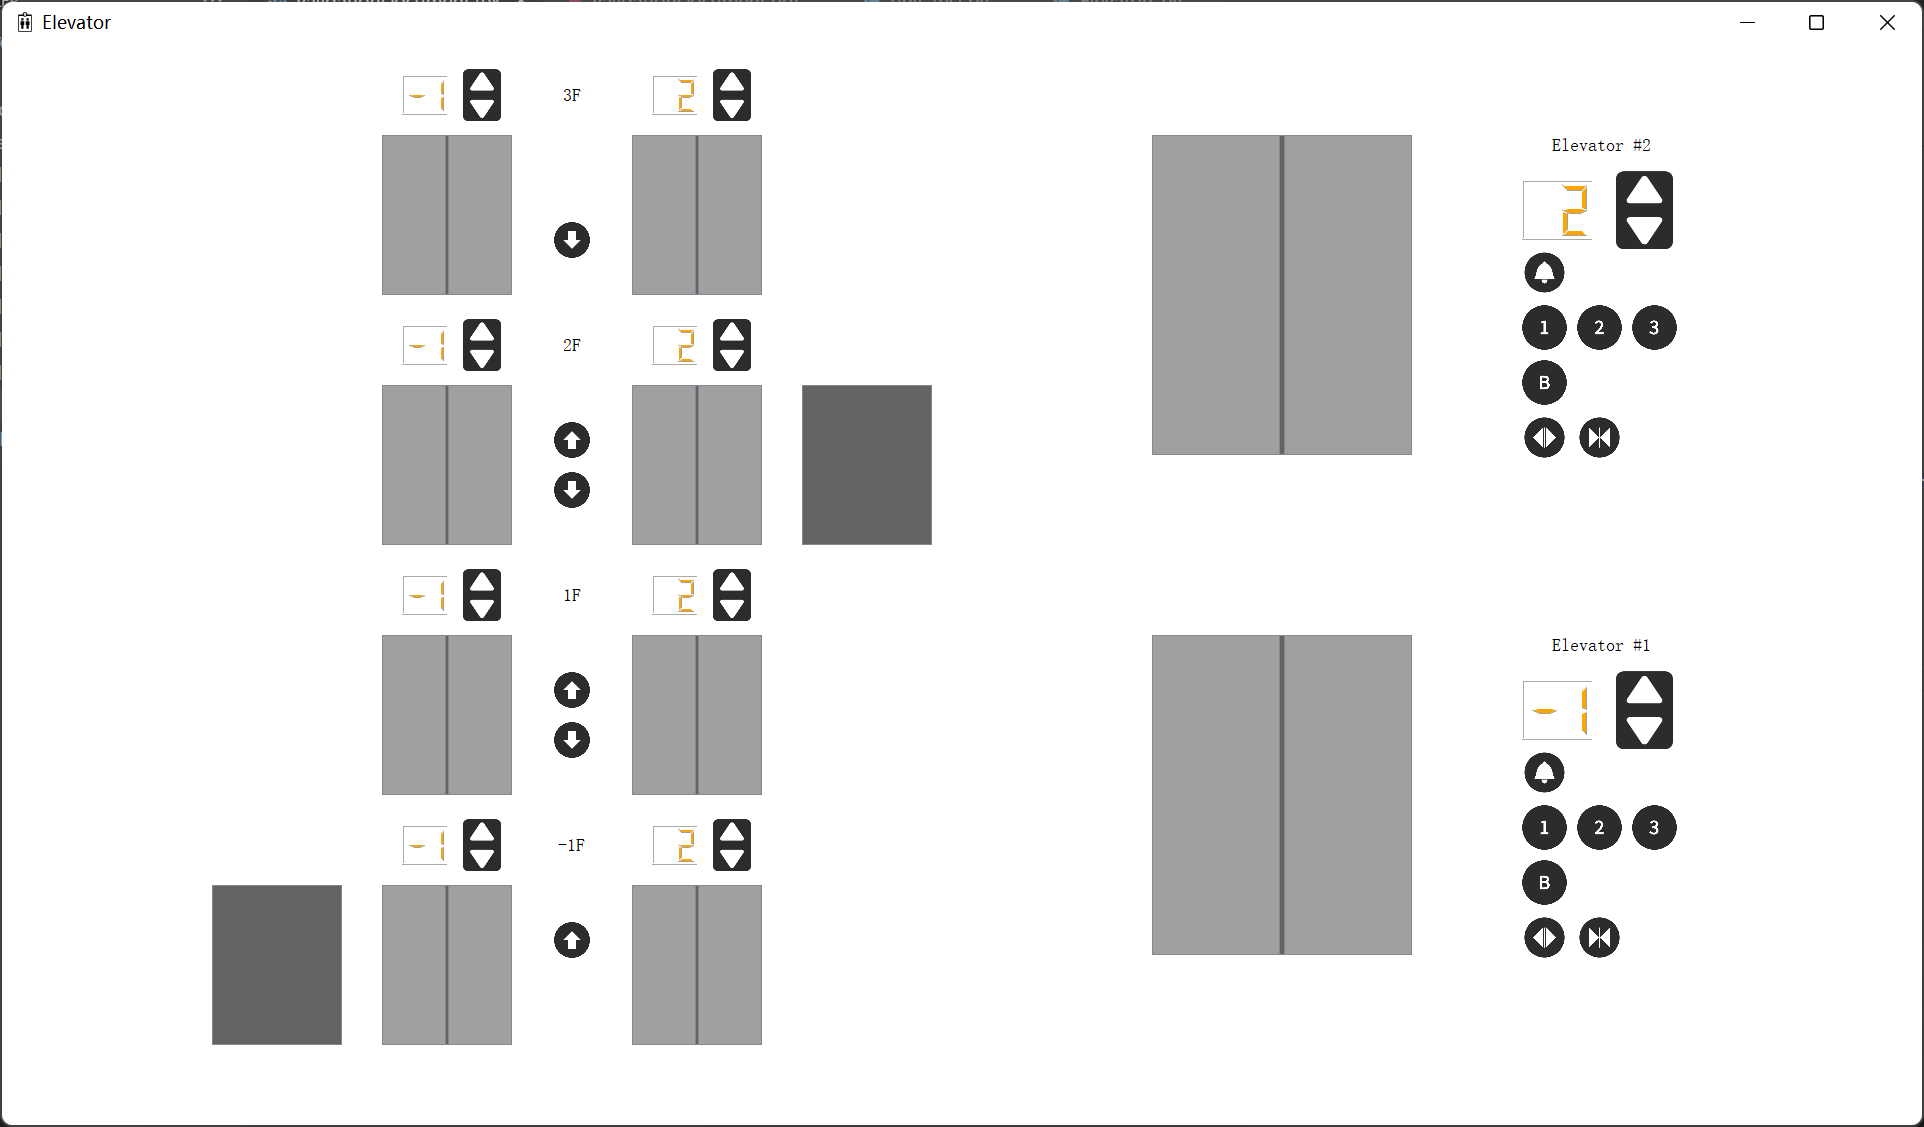
\includegraphics[width=0.8\textwidth]{img/T18.png}
    \caption{T18}
\end{figure}

\subsubsection*{T19: Button Display}
$\textbf{Purposes:}$ To check whether the button display changes correctly.

$\textbf{Test Results:}$ Randomly click on buttons many times, correct button colour display.

\begin{figure}[htbp]
    \centering
    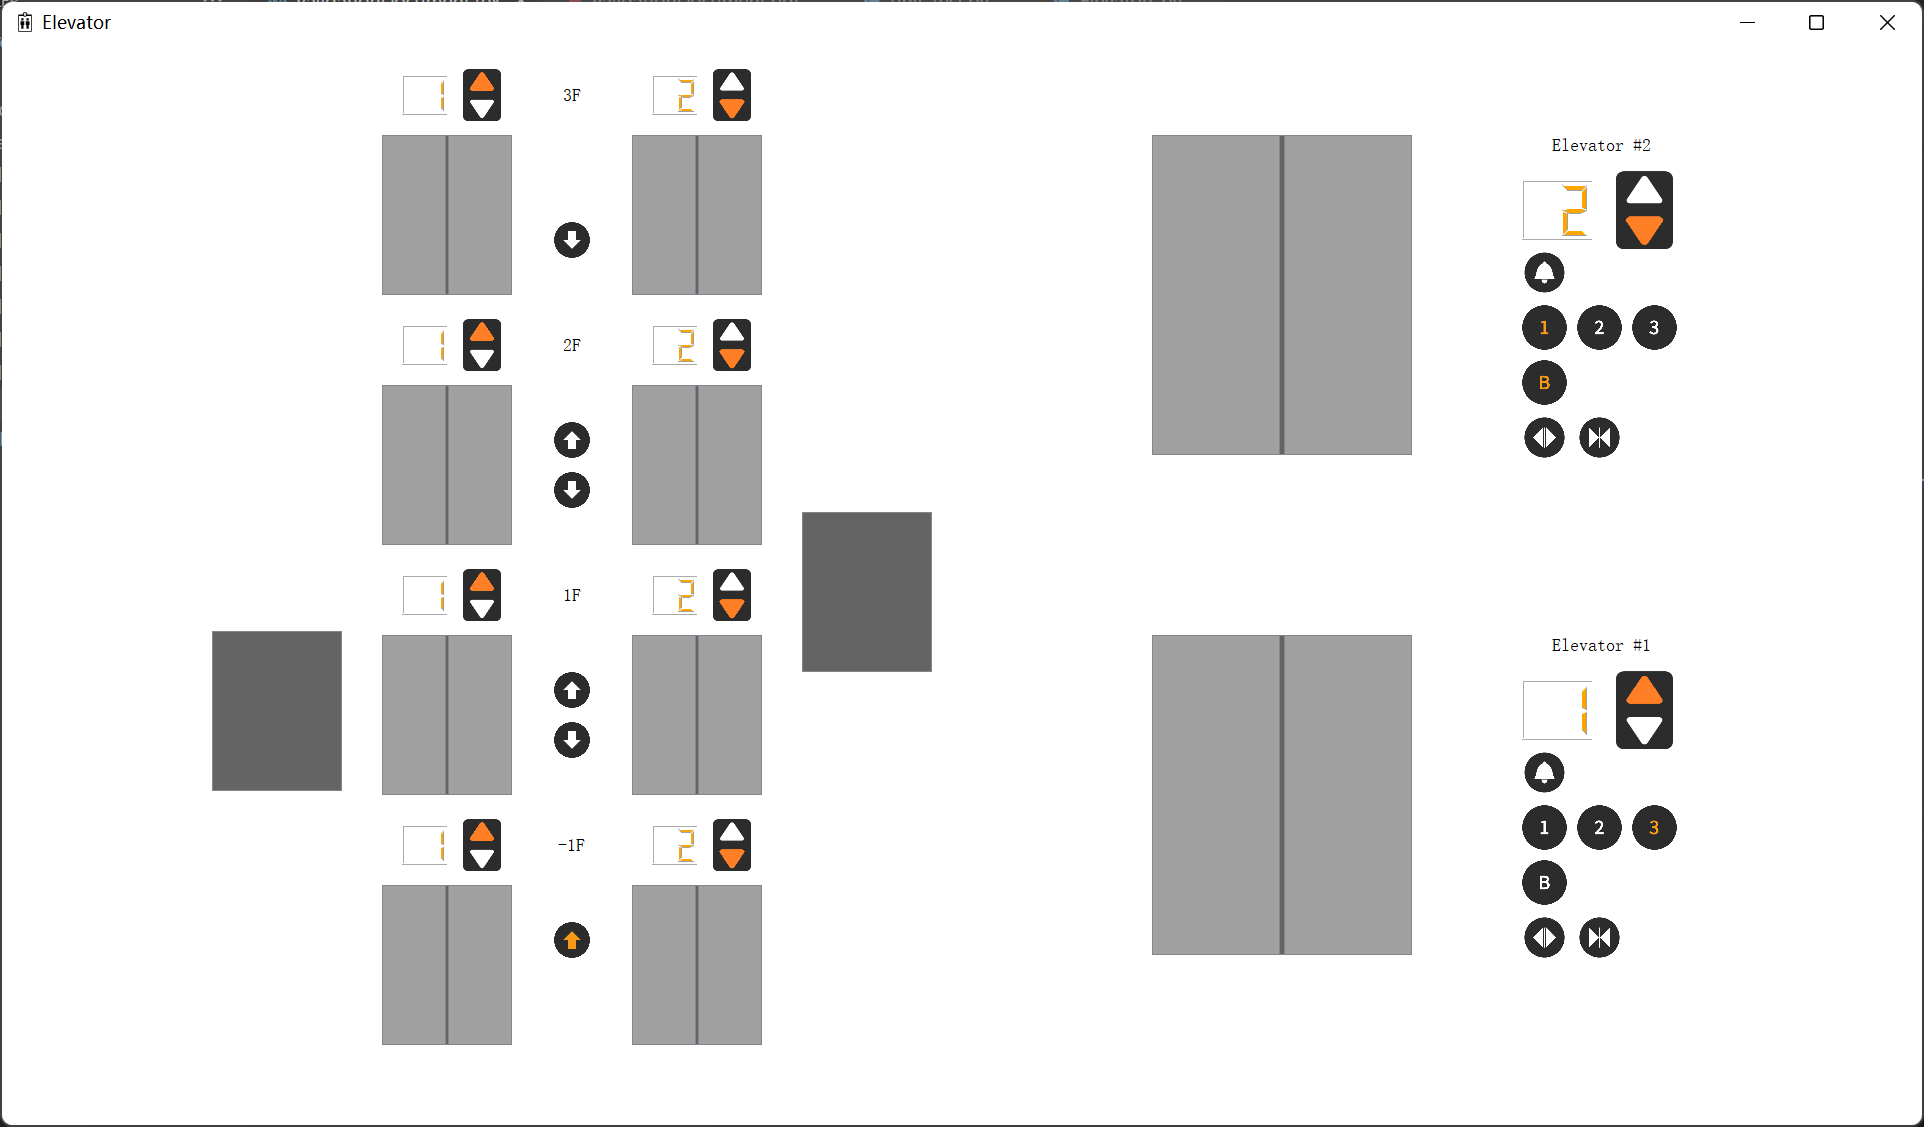
\includegraphics[width=0.8\textwidth]{img/T19.png}
    \caption{T19}
\end{figure}

\subsubsection*{T20: Direction Display}
$\textbf{Purposes:}$ To check whether the button elevator directions display correctly.

$\textbf{Test Results:}$ Randomly click on buttons many times, correct directions display and elevator direction correspondence.

\begin{figure}[htbp]
    \centering
    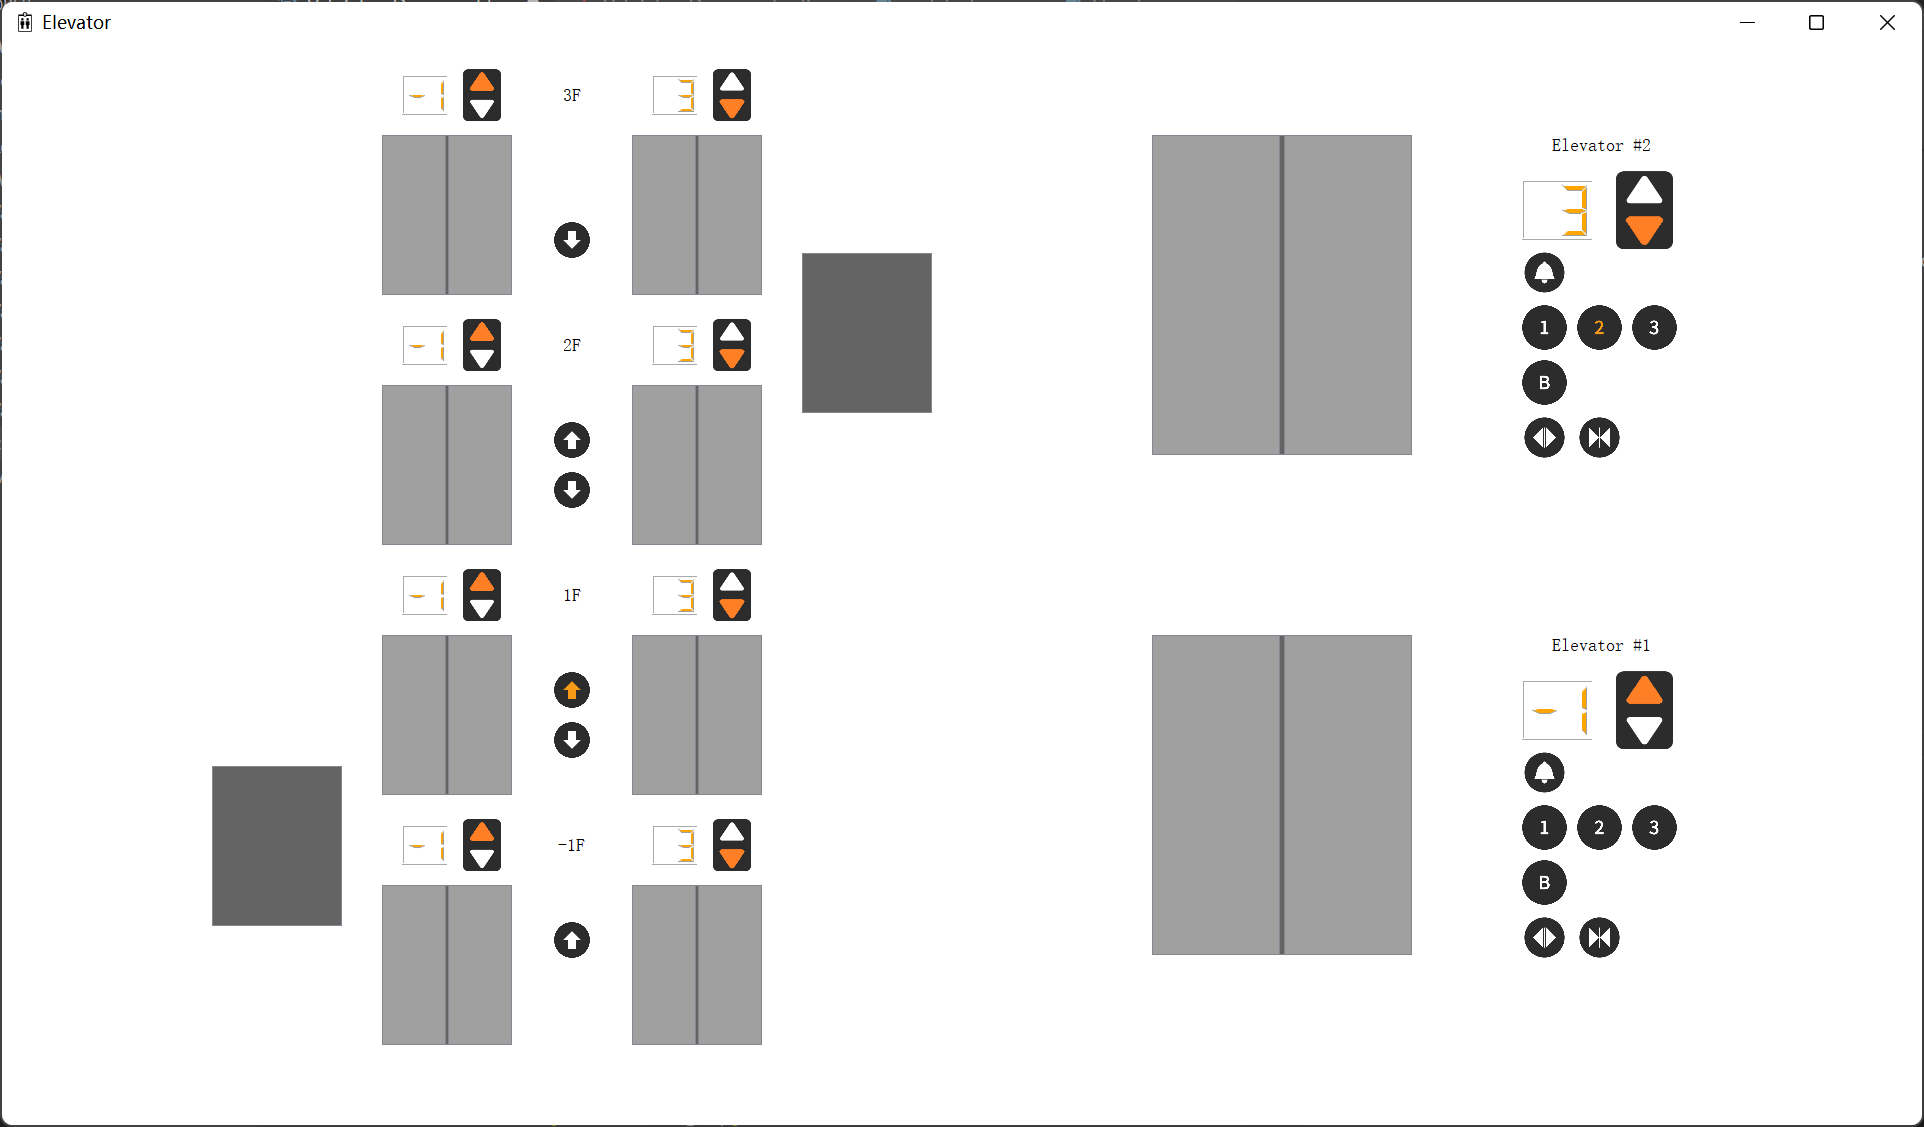
\includegraphics[width=0.8\textwidth]{img/T20.png}
    \caption{T20}
\end{figure}

\subsubsection*{T21: Door Animation Display}
$\textbf{Purposes:}$ To check whether the door open and close animations display correctly.

$\textbf{Test Results:}$ Correctly and it's continuous in order to allow door opening and closing without delay.

\begin{figure}[htbp]
    \centering
    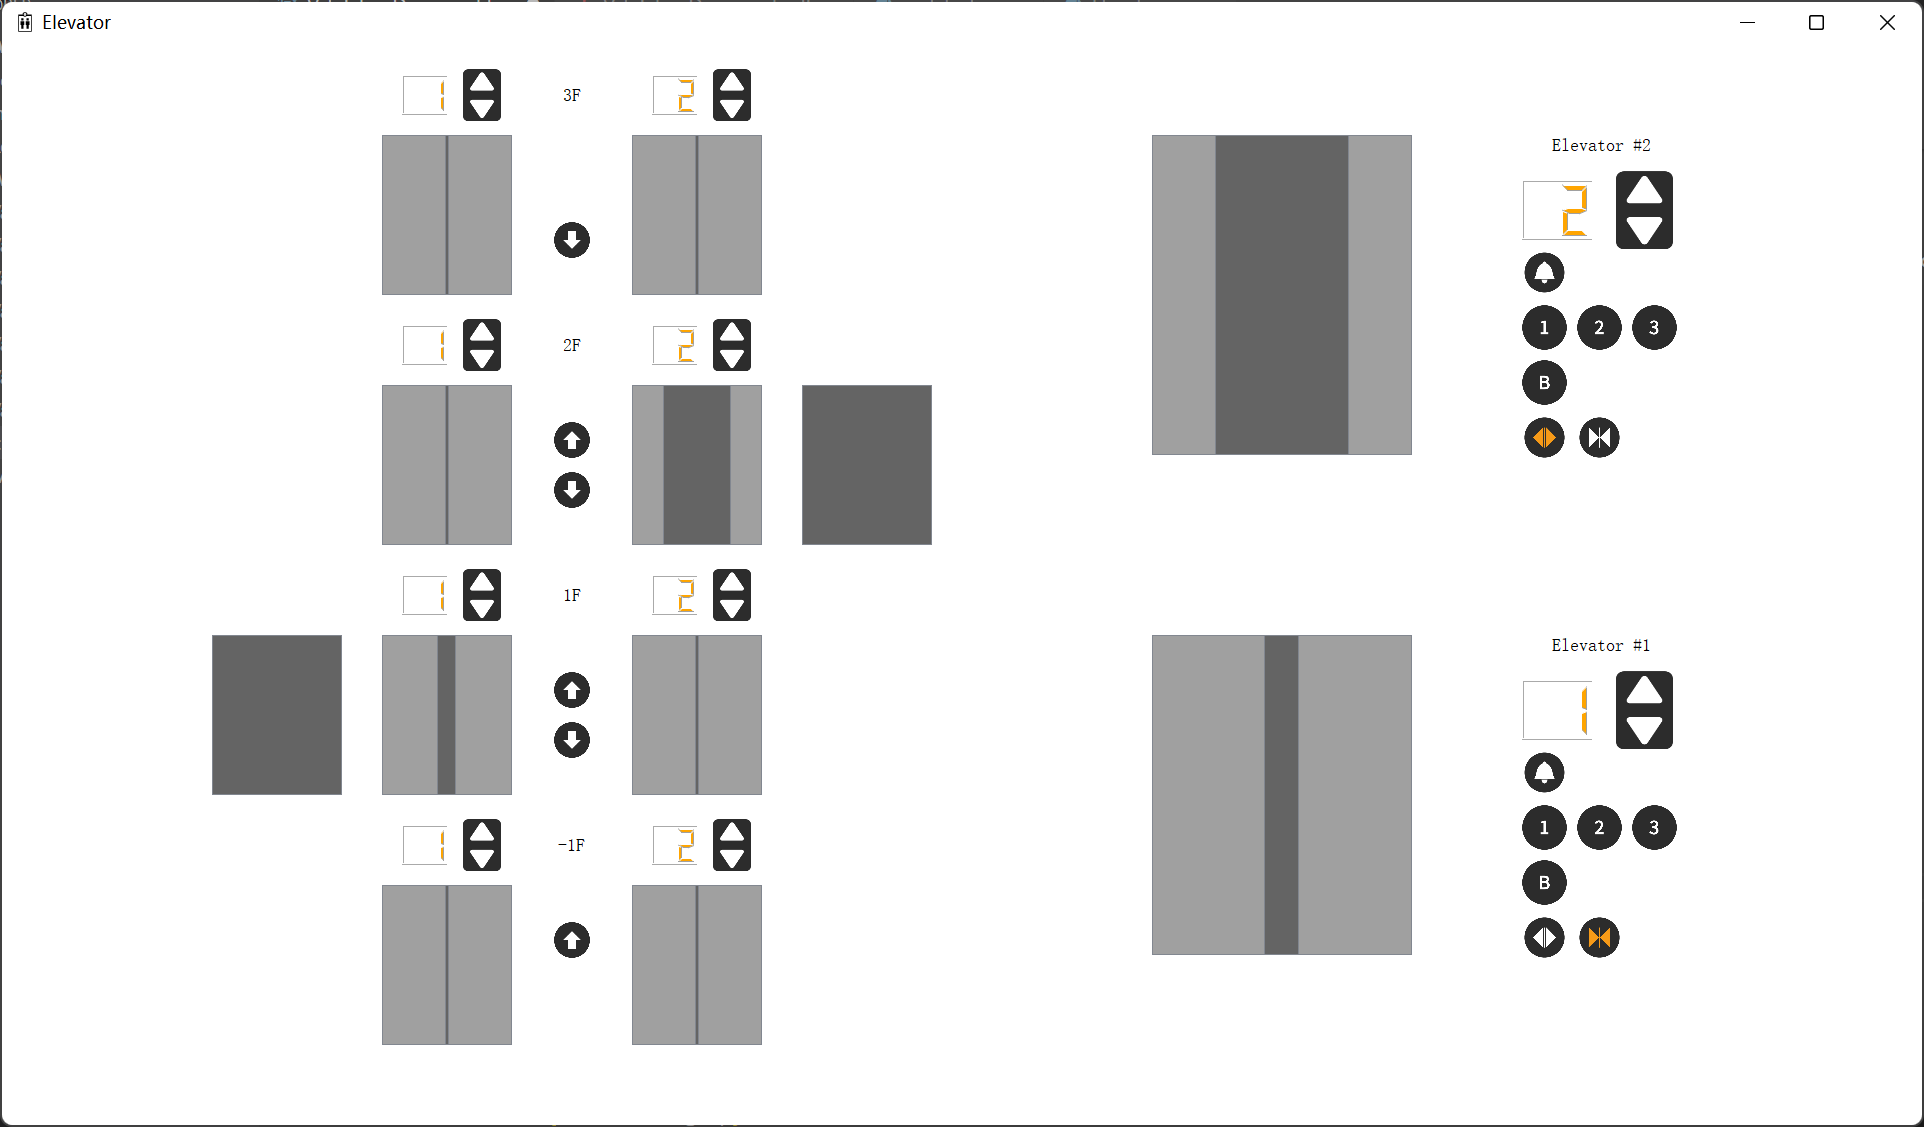
\includegraphics[width=0.8\textwidth]{img/T21.png}
    \caption{T21}
\end{figure}

\subsubsection*{T22: Moving Elevators Animation Display}
$\textbf{Purposes:}$ To check elevator moving animations display correct positions.

$\textbf{Test Results:}$ Correct.

\begin{figure}[htbp]
    \centering
    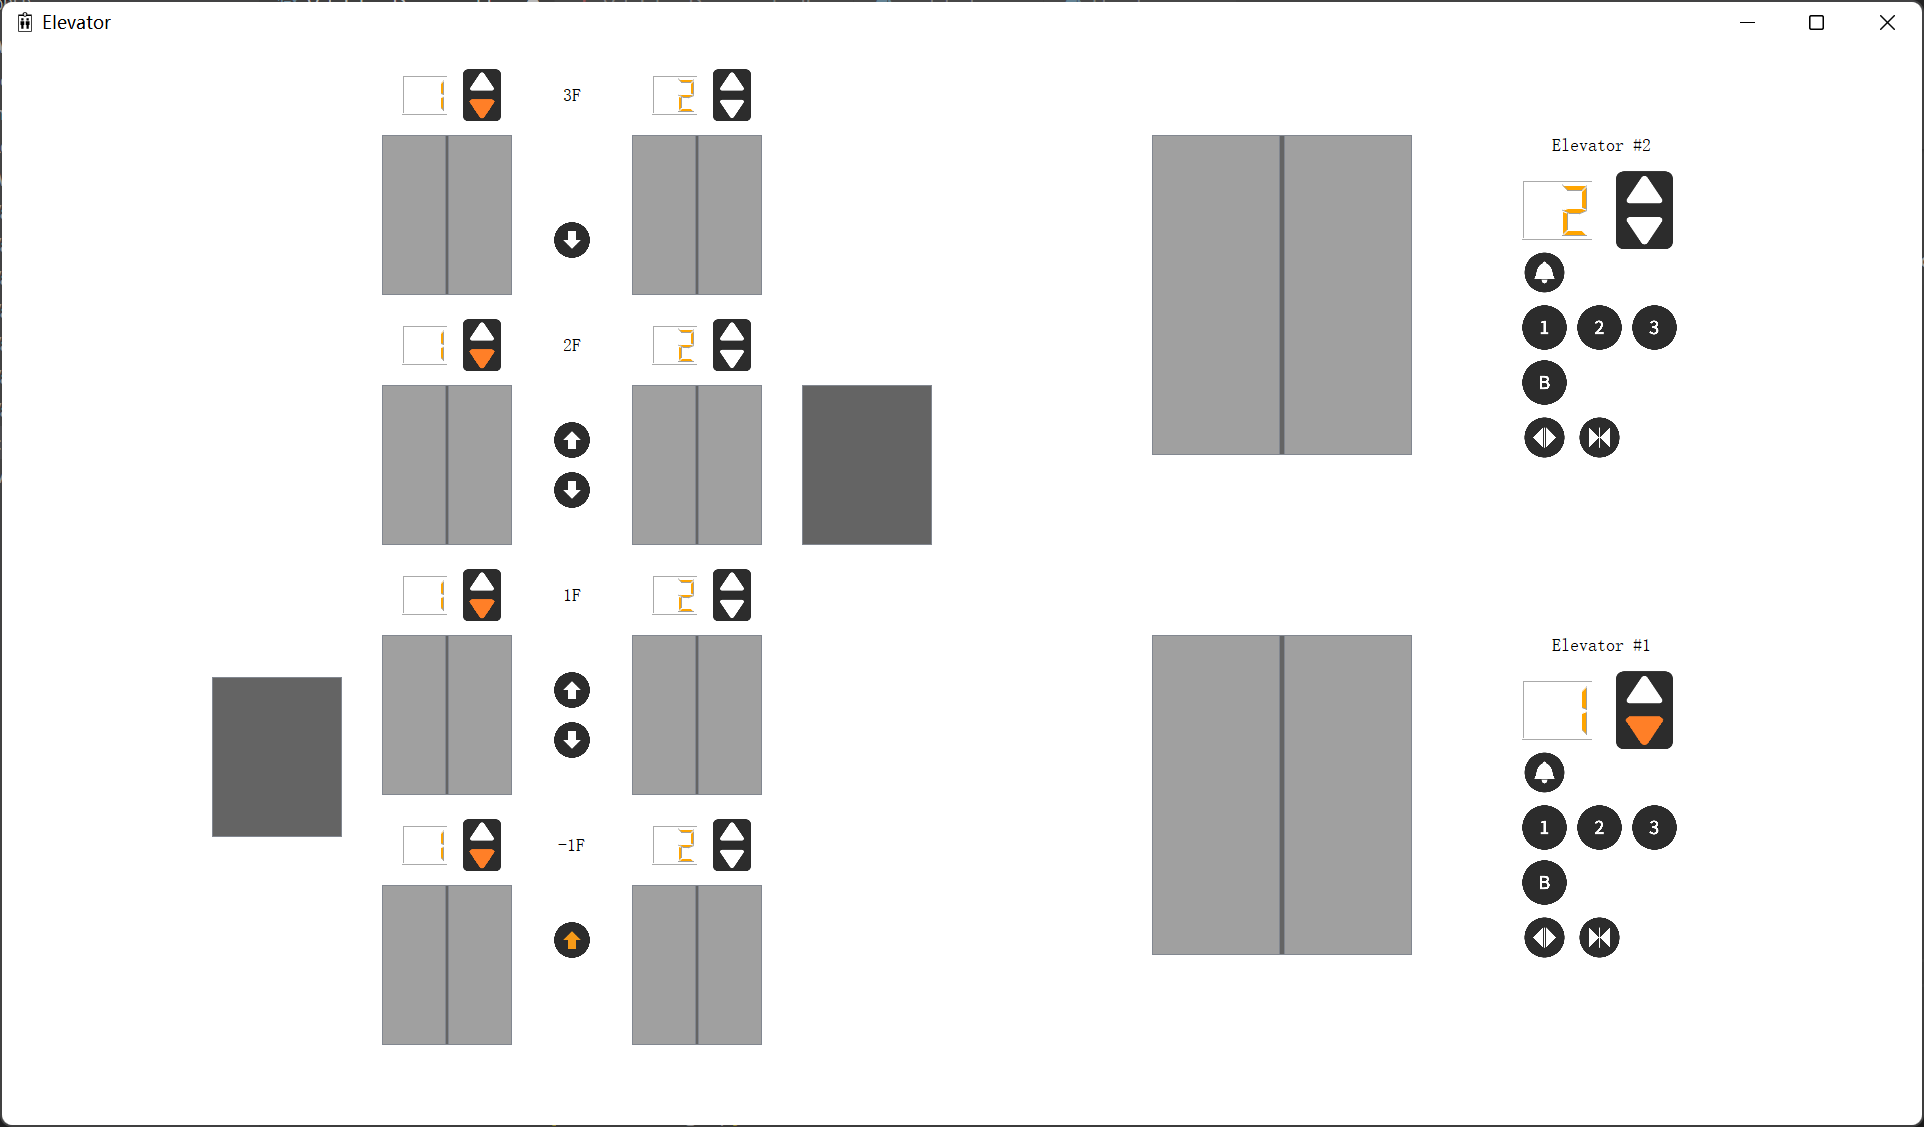
\includegraphics[width=0.8\textwidth]{img/T22.png}
    \caption{T22}
\end{figure}

\subsection*{Buttons}
\subsubsection*{T23: Calling up}
$\textbf{Purposes:}$ Test the call-up buttons in the interface.

$\textbf{Test Results:}$ Each simple call-up request will be handled in limited time.

\subsubsection*{T24: Calling down}
$\textbf{Purposes:}$ Test the call-down buttons in the interface.

$\textbf{Test Results:}$ Each simple call-down request will be handled in limited time.

\subsubsection*{T25: Inside floors}
$\textbf{Purposes:}$ Test the inside floor buttons of both elevators in the interface.

$\textbf{Test Results:}$ Each simple floor call request will be handled in limited time.

\subsubsection*{T26: Inside open and close}
$\textbf{Purposes:}$ Test the valid and invalid open and close.

$\textbf{Test Results:}$ Operation will be handled when stopping at a floor(valid), will not be handled when moving(invalid).

\subsubsection*{T27: Cancelling}
$\textbf{Purposes:}$ There is a lately added function: click on a clicked button again to cancel. Test its function correctness.

$\textbf{Test Results:}$ Will cancel the operation and stop at the following floor.

\newpage
\section{Integration Test}

Integration testing involves testing the interactions between different components or modules of a software application to ensure they work together correctly. This type of testing focuses on identifying issues that occur when integrating various parts of the system, such as data flow, interface compatibility, and overall interaction between modules. Integration tests help ensure that combined components function as expected, detect faults that may arise from module dependencies, and verify that the system's integrated parts operate smoothly together. This practice helps to uncover problems that unit tests might miss, ensuring a cohesive and reliable software system.

Here the integration tests include all the perspectives, including the dispatcher.

I will show by using commands similar but not same as that of API to show inputs and outputs.
\subsection*{T28}
\begin{lstlisting}
call-up@1
Re: open-close@1
select-floor3@2
select-floor2@2
Re: floor-arrived2@2
Re: floor-arrived3@2
call-down@1
Re: open-close@1
select-floorB@1
Re: floor-arrivedB@1
call-up@2
Re: floor-arrived2@2
\end{lstlisting}
$\textbf{Explanations:}$ The testcase mainly covers basic functions and dispatcher. First, from 1 to 3 when having not reached 2, press 2, the elevator will stop at 2.
Second, when both elevators are idle, regardless of the direction, the closer one will go and pick up passengers.

\subsection*{T29}
\begin{lstlisting}
call-up@B
Re: floor-arrived2@B
call-down@3
Wait for elevator 1 to move past floor2 but have not reached floor3
call-down@2
Re: floor-arrived1@3
Re: floor-arrived2@2
\end{lstlisting}
$\textbf{Explanations:}$ Apart from basic functions, this testcase verifies that from 1 to 3 when having reached 2 above, press 2, the elevator won't handle the command immediately.

\subsection*{T30}
\begin{lstlisting}
call-up@B
Re: floor-arrived2@B
select-floor3@1
call-down@2
Re: floor-arrived3@1
Re: floor-arrived2@2
select-floorB@1
Wait for elevator 1 to move past floor2 but have not reached floor3
select-floor2@1
Re: floor-arrivedB@1
Re: floor-arrived2@1  
\end{lstlisting}
$\textbf{Explanations:}$ Apart from basic functions, this case verifies invalid call from outside buttons.

\subsection*{T31}
\begin{lstlisting}
call-down@1
Re: open-close@2
select-floorB@2
Re: floor-arrivedB@2
call-up@1
Re: open-close@1
select-floor3@2
call-up@2
Re: floor-arrived2@1
Re: floor-arrived3@1
\end{lstlisting}
$\textbf{Explanations:}$ This case additionally verifies the dispatching processes when both elevators are moving.

\newpage
\section{Model Checking}

UPPAAL model checking involves using the UPPAAL tool to verify the correctness of real-time systems by creating and analyzing models of system behavior. This type of verification ensures that the system meets specified temporal properties and constraints, such as timing requirements and concurrency conditions. UPPAAL allows users to model systems using timed automata, simulate their behavior, and check properties expressed in temporal logic. This practice helps identify design flaws, verify system performance, and ensure that the system adheres to critical timing constraints, ultimately contributing to the development of reliable and robust real-time systems.

Here I use models that are not completely the same as that of development, but are similar to them. I use these simplified models to check some basic properties.
\subsection*{Risk Management}

1. Make sure each passenger that is picked up will be sent to target floor.

2. Make sure the elevator will not reach floors higher than 3 or lower than B.

3. Make sure each arrival to the following destination does not take too long.

$\textbf{FTA:}$

\begin{figure}[htbp]
    \centering
    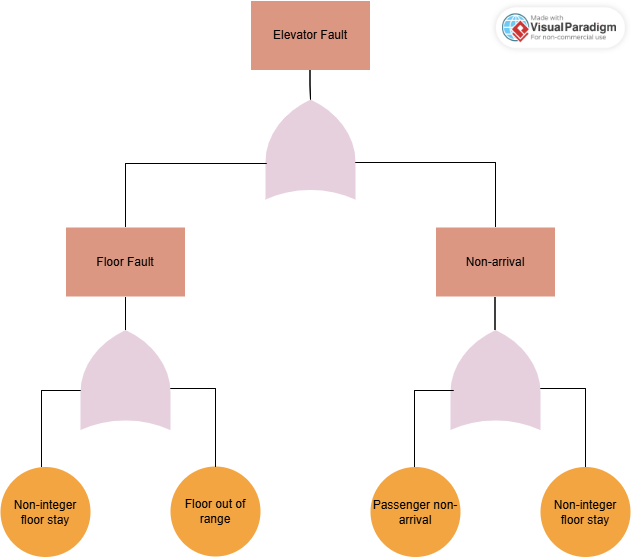
\includegraphics[width=0.25\textwidth]{img/ft.png}
    \caption{FTA}
\end{figure}
\subsection*{UPPAAL Models}
\subsubsection*{T32}
The first model assumes that there is only one elevator and passengers enter and exit the elevator in turn.

First define the system:\lstinline!ElevatorController!.

Define variables:
\begin{lstlisting}
int current_floor=1;
int out_button=-1;
int in_button=-1;
int minus_times=0;
int each_interval=0;
\end{lstlisting}
where \lstinline!minustimes! represents difference of pickups and sendings of passengers, \lstinline!each_interval! represents the time intervals between being picked and being sent.

Below is the state machine of UPPAAL:

\begin{figure}[htbp]
    \centering
    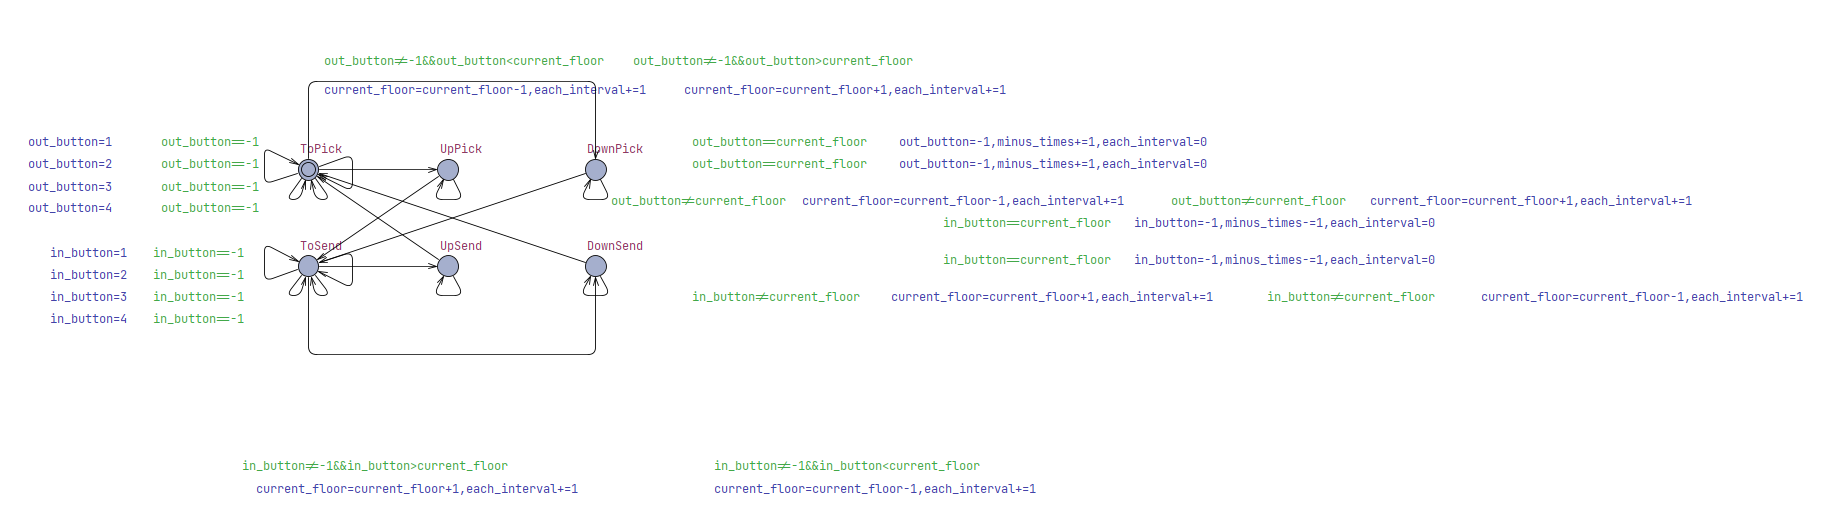
\includegraphics[width=\textwidth]{img/uppaal_state_machine_1.png}
    \caption{T32 State Machine}
\end{figure}

Below is the verifications:

\begin{figure}[htbp]
    \centering
    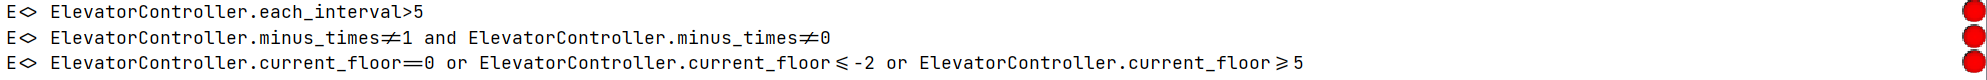
\includegraphics[width=\textwidth]{img/uppaal_verification_1.png}
    \caption{T32 Verification}
\end{figure}

The three verifications ensure the nonexistence of the three risks in this simplified model.

\subsubsection*{T33}
This models add the interactions between the elevator controller and the passengers. I add 4 passengers totally.

The first model assumes that there is only one elevator too, but passengers not necessarily enter and exit the elevator in turn.

Here is the system definition:
\begin{lstlisting}
passenger1 = Passenger();
passenger2 = Passenger();
passenger3 = Passenger();
passenger4 = Passenger();

system ElevatorController, passenger1,passenger2,passenger3,passenger4;
\end{lstlisting}

Controller variables remain unchanged and the global declarations:
\begin{lstlisting}
broadcast chan can_send, can_pick;
broadcast chan p1, p2, p3, p4;
broadcast chan s1, s2, s3, s4;

int interval=0;
\end{lstlisting}

Passengers and controller interact through the 8 $\textbf{broadcast chan}$s.

Below is the controller state machine:

\begin{figure}[htbp]
    \centering
    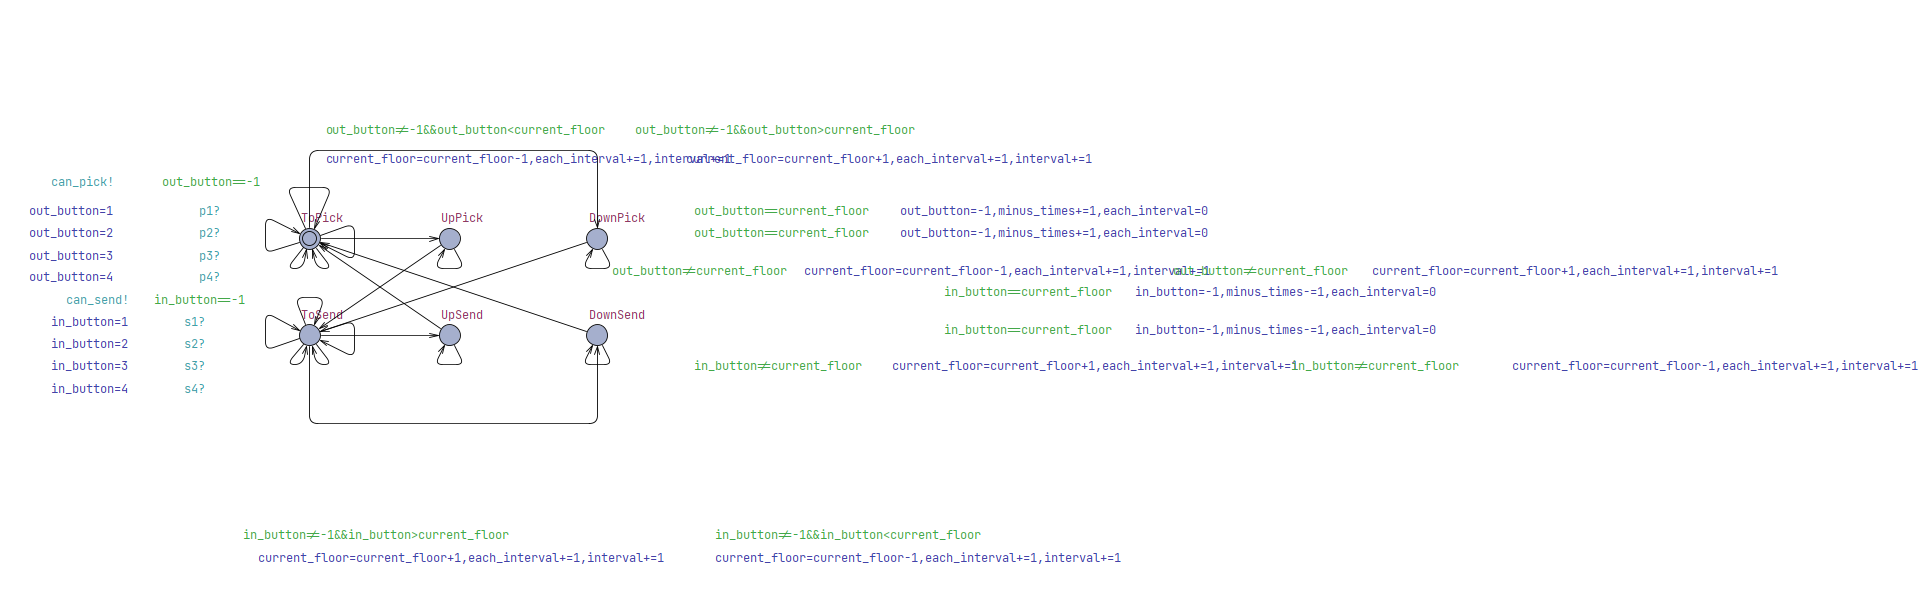
\includegraphics[width=\textwidth]{img/uppaal_controller_2.png}
    \caption{T33 Controller State Machine}
\end{figure}

Below is the passenger state machine:

\begin{figure}[htbp]
    \centering
    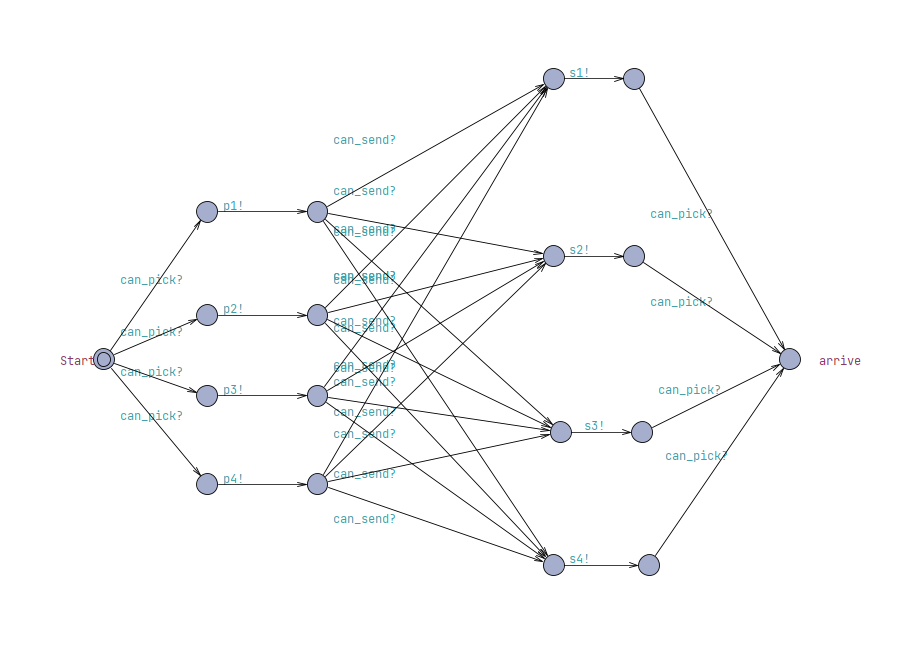
\includegraphics[width=\textwidth]{img/uppaal_passenger_2.png}
    \caption{T33 Passenger State Machine}
\end{figure}

Below is the verification:

\begin{figure}[htbp]
    \centering
    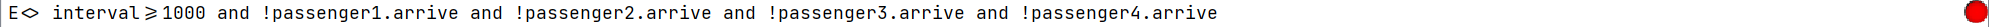
\includegraphics[width=\textwidth]{img/uppaal_verification_2.png}
    \caption{T33 Verification}
\end{figure}

We can see that we can always pick and send the four passengers within limited elevator state transfers.

\end{document}